\documentclass[%
  crop,%
  tikz,%
  multi=false%
]{standalone}%
\usepackage[utf8]{luainputenc}%
\usepackage[no-math]{fontspec}%
\defaultfontfeatures{%
  Numbers={OldStyle,Proportional},%
  Ligatures=TeX,%
  Extension=.ttf,%
}%
\setmainfont[%
  UprightFont=*-Regular,%
  ItalicFont=*-Italic,%
  BoldFont=*-Bold,%
  BoldItalicFont=*-BoldItalic,%
]{Raleway}%
\setsansfont[%
  UprightFont=*-Regular,%
  ItalicFont=*-Italic,%
  BoldFont=*-Bold,%
  BoldItalicFont=*-BoldItalic,%
]{Raleway}%
\usepackage[frenchmath]{mathastext}%
\usepackage{amsmath}%
\usepackage{amssymb}%
\usepackage{mathrsfs}%
\usepackage{mathtools}%
\usepackage{siunitx}%
\usepackage[siunitx]{circuitikz}%
\usetikzlibrary{calc,backgrounds,arrows.meta,patterns,positioning}%
\ctikzset{bipoles/length=1.2cm}%

% Colors
\usepackage{xcolor}%
\definecolor{RoseauGreen}{HTML}{cad40e}%
\definecolor{RoseauGrey}{HTML}{adb9cb}%
\definecolor{RoseauBlue}{HTML}{234e83}%

\DeclareMathOperator{\sign}{sign}%

% Sets
\let\C\relax
\newcommand{\R}{\ensuremath{\mathbb{R}}} % Real
\newcommand{\N}{\ensuremath{\mathbb{N}}} % Natural
% \newcommand{\C}{\ensuremath{\mathbb{C}}} % Complexes
\newcommand{\B}{\ensuremath{\mathscr{B}}} % Electrical buses
\newcommand{\Ch}{\ensuremath{\mathscr{C}}} % Loads
\renewcommand{\L}{\ensuremath{\mathscr{L}}} % Lines
\renewcommand{\P}{\ensuremath{\mathscr{P}}} % Phases

% Phases
\newcommand{\arm}{\ensuremath{\mathrm{a}}}%
\newcommand{\brm}{\ensuremath{\mathrm{b}}}%
\newcommand{\crm}{\ensuremath{\mathrm{c}}}%
\newcommand{\nrm}{\ensuremath{\mathrm{n}}}%
\newcommand{\grm}{\ensuremath{\mathrm{g}}}%
\newcommand{\abrm}{\ensuremath{\mathrm{ab}}}%
\newcommand{\bcrm}{\ensuremath{\mathrm{bc}}}%
\newcommand{\carm}{\ensuremath{\mathrm{ca}}}%
\newcommand{\anrm}{\ensuremath{\mathrm{an}}}%
\newcommand{\bnrm}{\ensuremath{\mathrm{bn}}}%
\newcommand{\cnrm}{\ensuremath{\mathrm{cn}}}%
\newcommand{\agrm}{\ensuremath{\mathrm{ag}}}%
\newcommand{\bgrm}{\ensuremath{\mathrm{bg}}}%
\newcommand{\cgrm}{\ensuremath{\mathrm{cg}}}%
\newcommand{\ngrm}{\ensuremath{\mathrm{ng}}}%
\newcommand{\abcrm}{\ensuremath{\mathrm{abc}}}%
\newcommand{\abcnrm}{\ensuremath{\mathrm{abcn}}}%

% Transformer
\newcommand{\Xrm}{\ensuremath{\mathrm{X}}}%
\newcommand{\Yrm}{\ensuremath{\mathrm{Y}}}%
\newcommand{\Zrm}{\ensuremath{\mathrm{Z}}}%
\newcommand{\xrm}{\ensuremath{\mathrm{x}}}%
\newcommand{\yrm}{\ensuremath{\mathrm{y}}}%
\newcommand{\zrm}{\ensuremath{\mathrm{z}}}%
\newcommand{\Arm}{\ensuremath{\mathrm{A}}}%
\newcommand{\Brm}{\ensuremath{\mathrm{B}}}%
\newcommand{\Crm}{\ensuremath{\mathrm{C}}}%
\newcommand{\Nrm}{\ensuremath{\mathrm{N}}}%

% Indices or exponents
\newcommand{\cons}{\ensuremath{\mathrm{cons.}}}%
\renewcommand{\prod}{\ensuremath{\mathrm{prod.}}}%
\newcommand{\theo}{\ensuremath{\mathrm{th.}}}%
\newcommand{\const}{\ensuremath{\mathrm{const.}}}%

% Variables
\newcommand{\umax}{\ensuremath{U^{\max}}}%
\newcommand{\umaxnorm}{\ensuremath{U^{\max\,\text{norm.}}}}%
\newcommand{\umin}{\ensuremath{U^{\min}}}%
\newcommand{\uminnorm}{\ensuremath{U^{\min\,\text{norm.}}}}%
\newcommand{\unom}{\ensuremath{U^{\text{nom.}}}}%
\newcommand{\unomnorm}{\ensuremath{U^{\text{nom.}\,\text{norm.}}}}%
\newcommand{\uup}{\ensuremath{U^{\text{up}}}}%
\newcommand{\uupnorm}{\ensuremath{U^{\text{up}\,\text{norm.}}}}%
\newcommand{\uupprime}{\ensuremath{U^{\text{up}\,\prime}}}%
\newcommand{\udown}{\ensuremath{U^{\text{down}}}}%
\newcommand{\udownnorm}{\ensuremath{U^{\text{down}\,\text{norm.}}}}%
\newcommand{\udownprime}{\ensuremath{U^{\text{down}\,\prime}}}%
\newcommand{\smax}{\ensuremath{S^{\max}}}%
\newcommand{\pmax}{\ensuremath{P^{\max}}}%
\newcommand{\sproj}{\ensuremath{\underline{S^{\text{proj.}}}}}%
%

\begin{document}
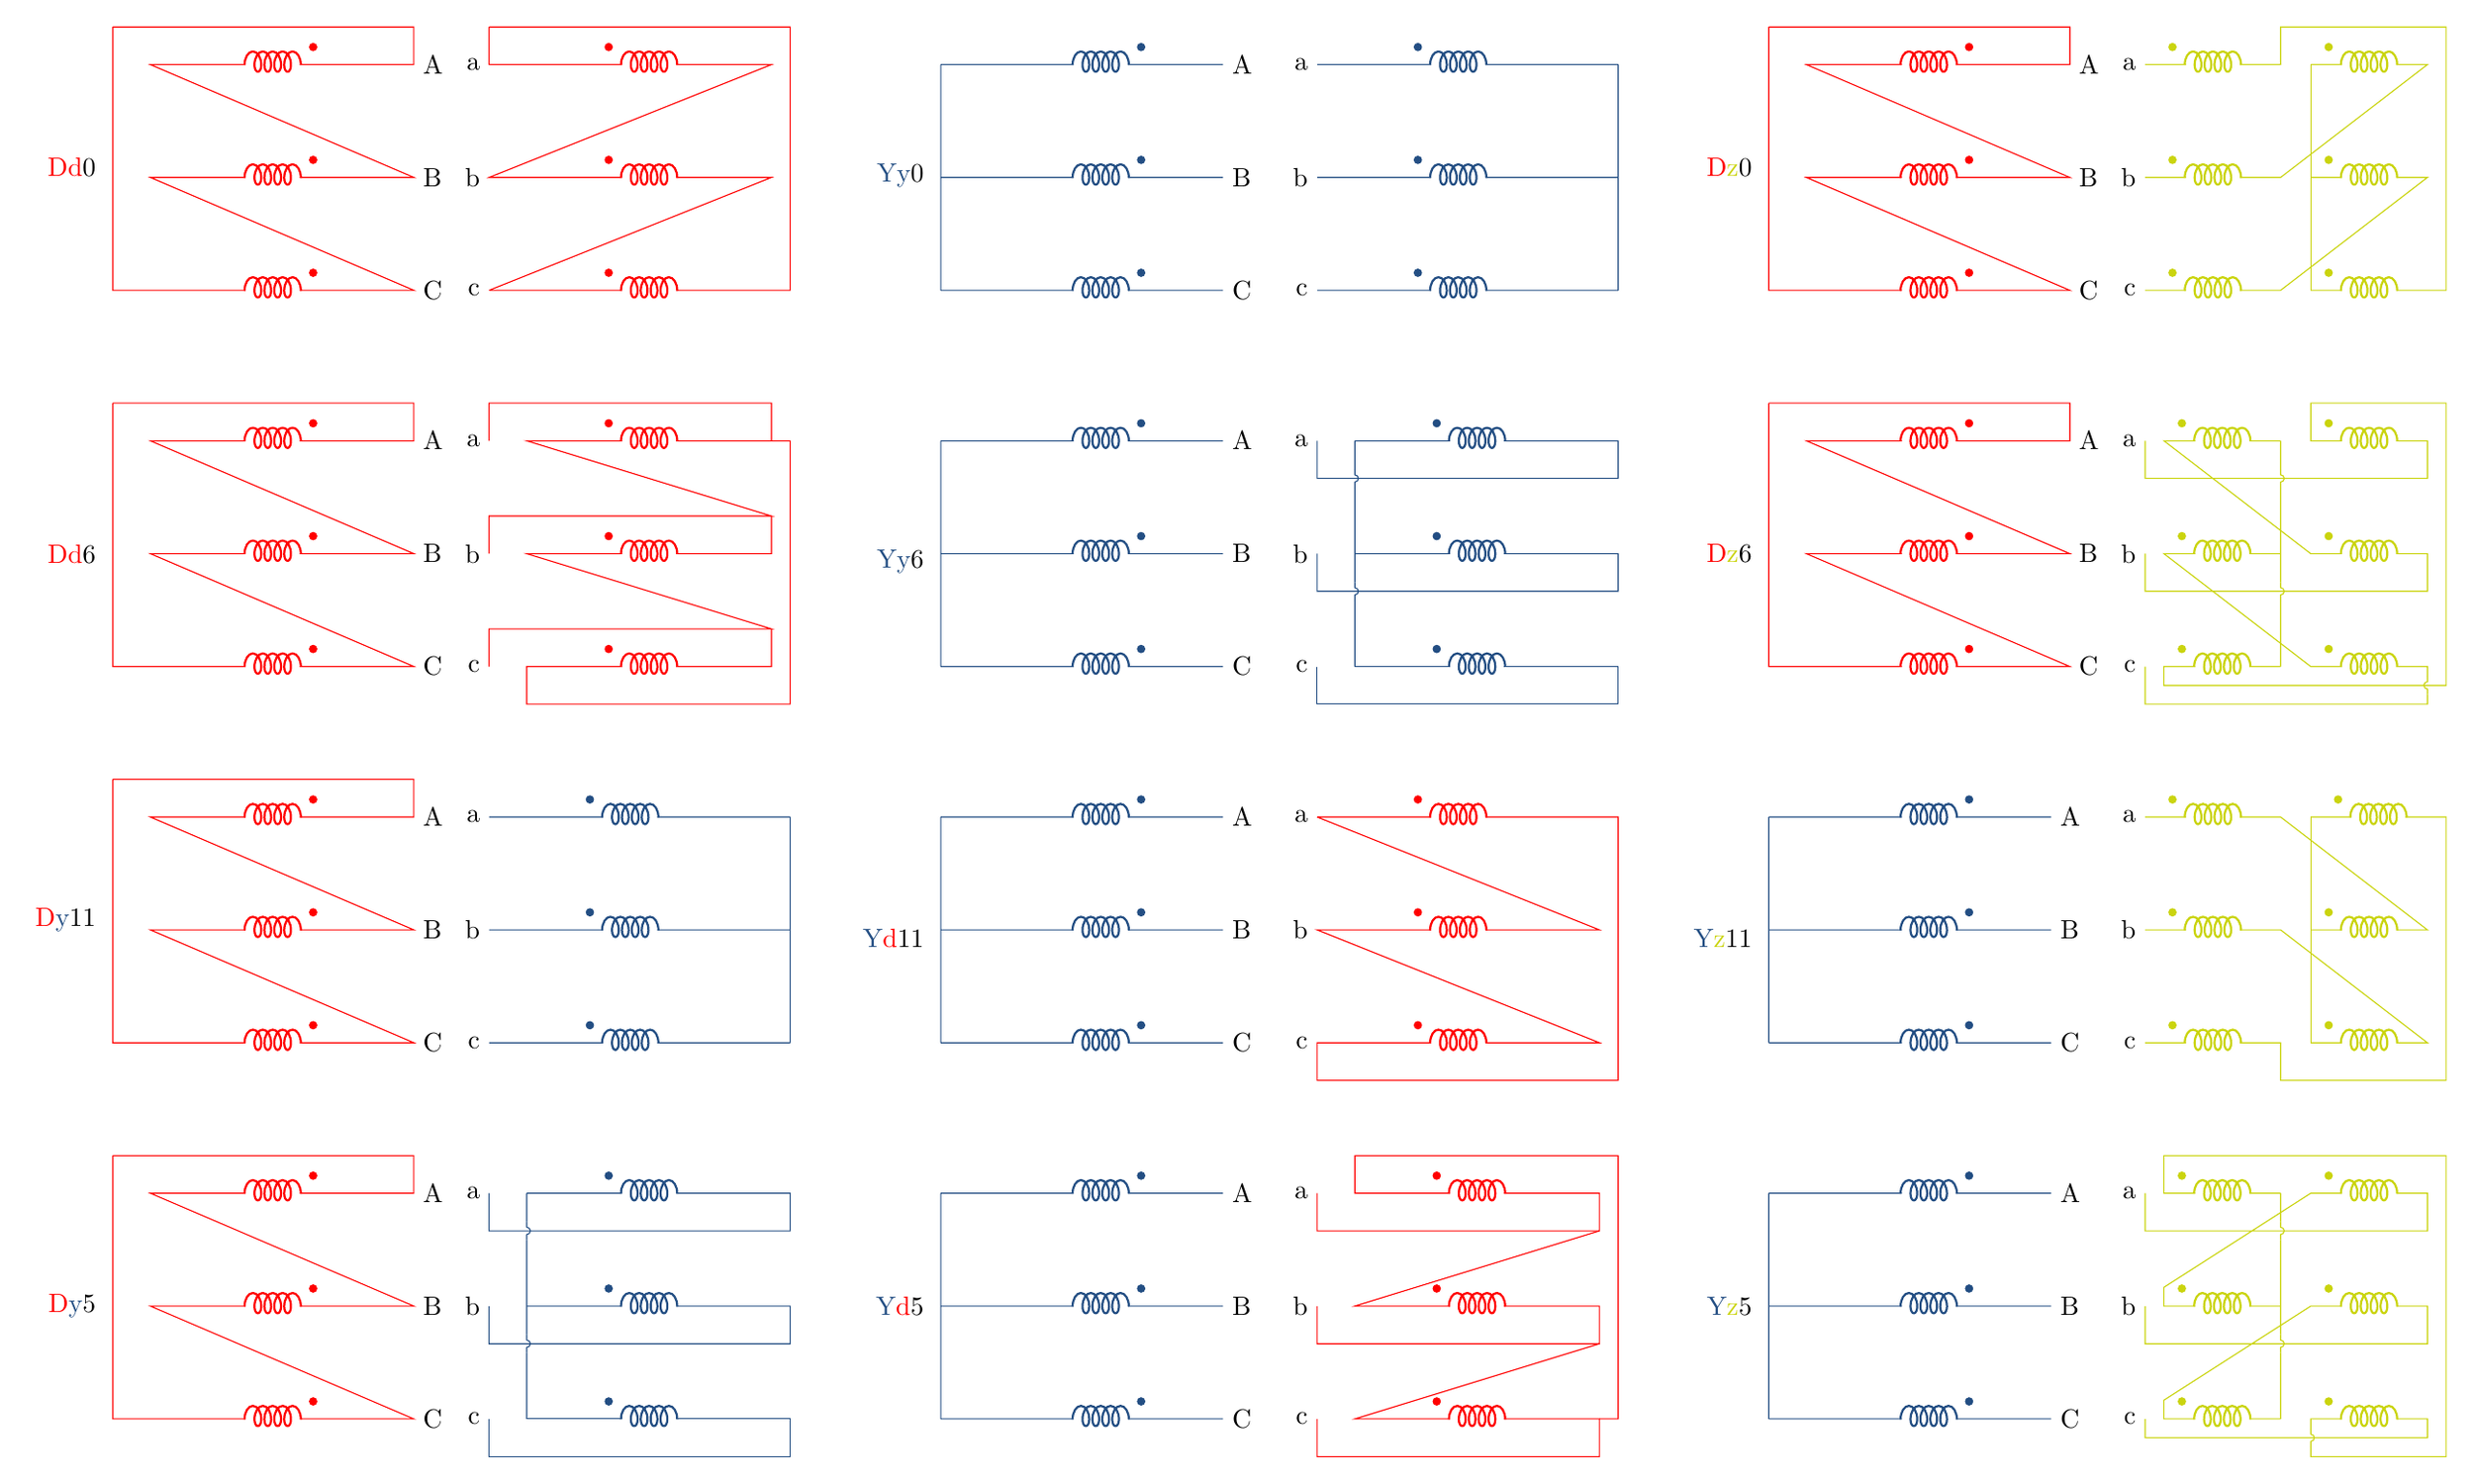
\begin{tikzpicture}[%
    show background rectangle,%
    tight background,%
    background rectangle/.style={fill=white}%
  ]
  %
% Definitions of windings
%
\pgfmathsetmacro{\yzero}{0}%
\pgfmathsetmacro{\yone}{-0.5}%
\pgfmathsetmacro{\ytwo}{-1}%
\pgfmathsetmacro{\ythree}{-1.5}%
\pgfmathsetmacro{\yfour}{-2}%
\pgfmathsetmacro{\yfive}{-2.5}%
\pgfmathsetmacro{\ysix}{-3}%
\pgfmathsetmacro{\yseven}{-3.5}%
\pgfmathsetmacro{\yeight}{-4}%

\pgfmathsetmacro{\xstep}{0.5}%
\pgfmathsetmacro{\xzero}{0}%
\pgfmathsetmacro{\xone}{0.25}%
\pgfmathsetmacro{\xtwo}{1.8}%
\pgfmathsetmacro{\xthree}{2}%
\pgfmathsetmacro{\xfour}{2.2}%
\pgfmathsetmacro{\xfive}{3.75}%
\pgfmathsetmacro{\xsix}{4}%

\ctikzset{european, straight voltages, bipoles/length=1.2cm, cute inductors}%

\tikzset{
  left d/.pic={
    \draw[red,text=black] (\xzero, \yzero) to[short, -] (\xsix, \yzero)%
    to[short, -]  (\xsix, \yone) node[right] {A}%
    to[short, -] (\xfive, \yone)%
    to[L, mirror, name=X] (\xstep, \yone)%
    to[short] (\xsix, \yfour) node[right] {B} %
    to[short, -] (\xfive, \yfour)%
    to[L, mirror, name=Y] (\xstep, \yfour) %
    to[short] (\xsix, \yseven) node[right] {C} %
    to[short, -] (\xfive, \yseven)%
    to[L, mirror, name=Z] (\xstep, \yseven) %
    to[short,-] (\xzero, \yseven) to[short,-] (\xzero, \yzero);%
    \path[fill=red,draw=red] (X.ul dot) node[circ]{}%
    (Y.ul dot) node[circ]{}%
    (Z.ul dot) node[circ]{};%
  },
  right d/.pic={
    \draw[red,text=black] (\xzero,0) to[short, -] (\xsix, \yzero)%
    to[short, -] (\xsix, \yseven)%
    to[short, -] (\xfive, \yseven)%
    to[L, mirror, name=z] (\xstep, \yseven)%
    to[short, -] (\xzero, \yseven) %
    to[short] (\xzero, \yseven) node[left] {c} %
    to[short, -] (\xfive, \yfour) %
    to[L, mirror, name=y] (\xstep, \yfour)%
    to[short, -] (\xzero, \yfour) node[left] {b} %
    to[short, -] (\xfive, \yone)%
    to[L, mirror, name=x] (\xstep, \yone) %
    to[short, -] (\xzero, \yone) node[left] {a} %
    to[short, -] (\xzero, \yzero);%
    \path[fill=red,draw=red] (x.ur dot) node[circ]{}%
    (y.ur dot) node[circ]{}%
    (z.ur dot) node[circ]{};%
  },
  right d6/.pic={
    \draw[red, text=black] (\xzero, \yone) node [left] {a}%
    to[short, -] (\xzero, \yzero)%
    to[short, -] (\xfive, \yzero) %
    to[short, -] (\xfive, \yone)%
    to[L, mirror, name=x] (\xstep, \yone)%
    to[short, -] (\xfive, \ythree)%
    to[short, -] (\xzero, \ythree)%
    to[short, -] (\xzero, \yfour) node[left] {b};%
    \draw[red, text=black] (\xfive, \ythree)%
    to[short, -] (\xfive, \yfour)%
    to[L, mirror, name=y] (\xstep, \yfour)%
    to[short, -] (\xfive, \ysix)%
    to[short, -] (\xzero, \ysix)%
    to[short, -] (\xzero, \yseven) node[left] {c};%
    \draw[red, text=black] (\xfive, \ysix)%
    to[short, -] (\xfive, \yseven)%
    to[L, mirror, name=z] (\xstep, \yseven)%
    to[short, -] (\xstep, \yeight)%
    to[short, -] (\xsix, \yeight)%
    to[short, -] (\xsix, \yone)
    to[short, -] (\xfive, \yone);%
    \path[fill=red,draw=red] (x.ur dot) node[circ]{}%
    (y.ur dot) node[circ]{}%
    (z.ur dot) node[circ]{};%
  },
  right d11/.pic={
    \draw[red, text=black] (\xzero, \yone) node [left] {a}%
    to[L, name=x] (\xfive, \yone)%
    to[short, -] (\xsix, \yone)%
    to[short, -] (\xsix, \yeight)%
    to[short, -] (\xzero, \yeight)%
    to[short, -] (\xzero, \yseven) node[left] {c}%
    to[L, name=z] (\xfive, \yseven)%
    to[short, -] (\xzero, \yfour) node[left] {b}%
    to[L, name=y] (\xfive, \yfour)%
    to[short, -] (\xzero, \yone);%
    \path[fill=red,draw=red] (x.ul dot) node[circ]{}%
    (y.ul dot) node[circ]{}%
    (z.ul dot) node[circ]{};%
  },
  right d5/.pic={
    \draw[red, text=black] (\xzero, \yone) node [left] {a}%
    to[short, -] (\xzero, \ytwo)%
    to[short, -] (\xfive, \ytwo)%
    to[short, -] (\xfive, \yone)%
    to[L, mirror, name=x] (\xstep, \yone)%
    to[short, -] (\xstep, \yzero)%
    to[short, -] (\xsix, \yzero)%
    to[short, -] (\xsix, \yseven)%
    to[short, -] (\xfive, \yseven);%
    \draw[red, text=black] (\xzero, \yfour) node [left] {b}%
    to[short, -] (\xzero, \yfive)%
    to[short, -] (\xfive, \yfive)%
    to[short, -] (\xfive, \yfour)%
    to[L, mirror, name=y] (\xstep, \yfour)%
    to[short, -] (\xfive, \ytwo);%
    \draw[red, text=black] (\xzero, \yseven) node [left] {c}%
    to[short, -] (\xzero, \yeight)%
    to[short, -] (\xfive, \yeight)%
    to[short, -] (\xfive, \yseven)%
    to[L, mirror, name=z] (\xstep, \yseven)%
    to[short, -] (\xfive, \yfive);%
    \path[fill=red,draw=red] (x.ur dot) node[circ]{}%
    (y.ur dot) node[circ]{}%
    (z.ur dot) node[circ]{};%
  },
  left y/.pic={
    \draw[RoseauBlue, text=black] (\xzero, \yone) to[short, -] (\xstep, \yone)%
    to[L, -, name=X] (\xfive, \yone) node[right] {A}%
    (\xzero,\yfour) to[short, -] (\xstep, \yfour)%
    to[L, -, name=Y]  (\xfive, \yfour) node[right] {B}%
    (\xzero,\yseven) to[short, -] (\xstep, \yseven)%
    to[L, -, name=Z]  (\xfive, \yseven) node[right] {C}%
    (\xzero,\yone) to[short, -] (\xzero,\yseven);%
    \path[fill=RoseauBlue,draw=RoseauBlue] (X.ur dot) node[circ]{}%
    (Y.ur dot) node[circ]{}%
    (Z.ur dot) node[circ]{};%
  },
  right y/.pic={
    \draw[RoseauBlue,text=black] (\xsix, \yone) to[short, -] (\xfive, \yone)%
    to[L, -, mirror, name=x] (\xzero, \yone) node[left] {a}%
    (\xsix, \yfour) to[short, -] (\xfive, \yfour)%
    to[L, -, mirror, name=y]  (\xzero,\yfour) node[left] {b}%
    (\xsix, \yseven) to[short, -] (\xfive, \yseven)%
    to[L, -, mirror, name=z]  (\xzero,\yseven) node[left] {c}
    (\xsix,\yone) to[short, -] (\xsix,\yseven);%
    \path[fill=RoseauBlue,draw=RoseauBlue] (x.ur dot) node[circ]{}%
    (y.ur dot) node[circ]{}%
    (z.ur dot) node[circ]{};%
  },
  right y reverse/.pic={
    \draw[RoseauBlue, text=black] (\xzero, \yone) node[left] {a} %
    to[short, -] (\xzero, \ytwo)%
    to[short, -] (\xsix, \ytwo)%
    to[short, -] (\xsix, \yone)%
    to[short, -] (\xfive, \yone)%
    to[L, -, mirror, name=x] (\xstep,\yone);%
    \draw[RoseauBlue, text=black] (\xzero, \yfour) node[left] {b} %
    to[short, -] (\xzero, \yfive)%
    to[short, -] (\xsix, \yfive)%
    to[short, -] (\xsix, \yfour)%
    to[short, -] (\xfive, \yfour)%
    to[L, -, mirror, name=y] (\xstep,\yfour);%
    \draw[RoseauBlue, text=black] (\xzero, \yseven) node[left] {c} %
    to[short, -] (\xzero, \yeight)%
    to[short, -] (\xsix, \yeight)%
    to[short, -] (\xsix, \yseven)%
    to[short, -] (\xfive, \yseven)%
    to[L, -, mirror, name=z] (\xstep,\yseven);%
    \draw[RoseauBlue] (\xstep, \yone) to[crossing] (\xstep, \ythree)%
    to[short, -] (\xstep, \yfour)%
    to[crossing] (\xstep, \ysix)%
    to[short, -] (\xstep, \yseven);%
    \path[fill=RoseauBlue,draw=RoseauBlue] (x.ur dot) node[circ]{}%
    (y.ur dot) node[circ]{}%
    (z.ur dot) node[circ]{};%
  },
  right z0/.pic={
    \draw[RoseauGreen, text=black] (\xzero, \yone) node[left] {a} %
    to[L, name=x1] (\xtwo, \yone)%
    to[short, -] (\xtwo,0)%
    to[short, -] (\xsix,0)%
    to[short, -] (\xsix,\yseven)%
    to[short, -] (\xfive,\yseven)%
    to[L, mirror, name=z2] (\xfour, \yseven);%
    \draw[RoseauGreen, text=black] (\xzero, \yfour) node[left] {b} %
    to[L, name=y1] (\xtwo, \yfour)%
    to[short, -] (\xfive, \yone)%
    to[L, mirror, name=x2] (\xfour, \yone);%
    \draw[RoseauGreen, text=black] (\xzero, \yseven) node[left] {c} %
    to[L, name=z1] (\xtwo, \yseven)%
    to[short, -] (\xfive, \yfour)%
    to[L, mirror, name=y2] (\xfour, \yfour);%
    \draw[RoseauGreen, text=black] (\xfour, \yseven) to[short, -] (\xfour, \yfour) to[short, -] (\xfour, \yone);
    \path[fill=RoseauGreen,draw=RoseauGreen] (x1.ul dot) node[circ]{}%
    (x2.ur dot) node[circ]{}%
    (y1.ul dot) node[circ]{}%
    (y2.ur dot) node[circ]{}%
    (z1.ul dot) node[circ]{}%
    (z2.ur dot) node[circ]{};%
  },
  right z6/.pic={
    \draw[RoseauGreen, text=black] (\xzero, \yone) node[left] {a} %
    to[short, -] (\xzero,\ytwo)%
    to[short, -] (\xfive, \ytwo)%
    to[short, -] (\xfive, \yone)%
    to[L, mirror, name=x2] (\xfour, \yone)%
    to[short, -](\xfour, 0)%
    to[short, -] (\xfive, 0)%
    to[short, -] (\xsix, 0)%
    to[short, -] (\xsix, \yseven-0.25)%
    to[short, -] (\xone, \yseven-0.25)%
    to[short, -] (\xone, \yseven)%
    to[L, name=z1] (\xtwo, \yseven);%
    \draw[RoseauGreen, text=black] (\xzero, \yfour) node[left] {b} %
    to[short, -] (\xzero,\yfive)%
    to[short, -] (\xfive, \yfive)%
    to[short, -] (\xfive, \yfour)%
    to[L, mirror, name=y2] (\xfour, \yfour)%
    to[short, -] (\xone, \yone)%
    to[L, name=x1] (\xtwo, \yone);%
    \draw[RoseauGreen, text=black] (\xzero, \yseven) node[left] {c} %
    to[short, -] (\xzero,\yeight)%
    to[short, -] (\xfive, \yeight)%
    to[crossing] (\xfive, \yseven)%
    to[L, mirror, name=z2] (\xfour, \yseven)%
    to[short, -] (\xone, \yfour)%
    to[L, name=y1] (\xtwo, \yfour);%
    \draw[RoseauGreen] (\xtwo, \yone) to[crossing] (\xtwo, \ythree)%
    to[short, -] (\xtwo, \yfour)%
    to[crossing] (\xtwo, \ysix)
    to[short, -] (\xtwo, \yseven);%
    \path[fill=RoseauGreen,draw=RoseauGreen] (x1.ul dot) node[circ]{}%
    (x2.ur dot) node[circ]{}%
    (y1.ul dot) node[circ]{}%
    (y2.ur dot) node[circ]{}%
    (z1.ul dot) node[circ]{}%
    (z2.ur dot) node[circ]{};%
  },
  right z11/.pic={
    \draw[RoseauGreen, text=black] (\xzero, \yone) node[left] {a} %
    to[L, name=x1] (\xtwo, \yone)%
    to[short, -] (\xfive, \yfour)%
    to[L, mirror, name=y2] (\xfour, \yfour);%
    \draw[RoseauGreen, text=black] (\xzero, \yfour) node[left] {b} %
    to[L, name=y1] (\xtwo, \yfour)%
    to[short, -] (\xfive, \yseven)%
    to[L, mirror, name=z2] (\xfour, \yseven);%
    \draw[RoseauGreen, text=black] (\xzero, \yseven) node[left] {c} %
    to[L, name=z1] (\xtwo, \yseven)%
    to[short, -] (\xtwo, \yeight)%
    to[short, -] (\xsix, \yeight)%
    to[short, -] (\xsix, \yone)%
    to[L, mirror, name=x2] (\xfour, \yone);%
    \draw[RoseauGreen] (\xfour, \yone) to[short] (\xfour, \yfour) to[short] (\xfour, \yseven);%
    \path[fill=RoseauGreen,draw=RoseauGreen] (x1.ul dot) node[circ]{}%
    (x2.ur dot) node[circ]{}%
    (y1.ul dot) node[circ]{}%
    (y2.ur dot) node[circ]{}%
    (z1.ul dot) node[circ]{}%
    (z2.ur dot) node[circ]{};%
  },
  right z5/.pic={
    \draw[RoseauGreen, text=black] (\xzero, \yone) node[left] {a} %
    to[short, -] (\xzero, \ytwo)%
    to[short, -] (\xfive, \ytwo)%
    to[short, -] (\xfive, \yone)%
    to[L, mirror, name=x2] (\xfour, \yone)%
    to[short, -] (\xone, \yfour+0.25)%
    to[short, -] (\xone, \yfour)%
    to[L, name=y1] (\xtwo, \yfour);%
    \draw[RoseauGreen, text=black] (\xzero, \yfour) node[left] {b} %
    to[short, -] (\xzero, \yfive)%
    to[short, -] (\xfive, \yfive)%
    to[short, -] (\xfive, \yfour)%
    to[L, mirror, name=y2] (\xfour, \yfour)%
    to[short, -] (\xone, \yseven+0.25)%
    to[short, -] (\xone, \yseven)%
    to[L, name=z1] (\xtwo, \yseven);%
    \draw[RoseauGreen, text=black] (\xzero, \yseven) node[left] {c} %
    to[short, -] (\xzero, \yseven-0.25)%
    to[short, -] (\xfive, \yseven-0.25)%
    to[short, -] (\xfive, \yseven)%
    to[L, mirror, name=z2] (\xfour, \yseven)%
    to[crossing] (\xfour, \yeight)%
    to[short, -] (\xsix, \yeight)%
    to[short, -] (\xsix, 0)%
    to[short, -] (\xone, 0)
    to[short, -] (\xone, \yone)%
    to[L, name=x1] (\xtwo, \yone);%
    \draw[RoseauGreen] (\xtwo, \yone) to[crossing] (\xtwo, \ythree)%
    to[short, -] (\xtwo, \yfour)%
    to[crossing] (\xtwo, \ysix)%
    to[short, -] (\xtwo, \yseven);%
    \path[fill=RoseauGreen,draw=RoseauGreen] (x1.ul dot) node[circ]{}%
    (x2.ur dot) node[circ]{}%
    (y1.ul dot) node[circ]{}%
    (y2.ur dot) node[circ]{}%
    (z1.ul dot) node[circ]{}%
    (z2.ur dot) node[circ]{};%
  }
}
%

  % Phase displacement = 0
  \begin{scope}[local bounding box=Dd0]
    \pic at (0,0) {left d};%
    \pic at (5,0) {right d};%
  \end{scope}
  \node[left=0.1 of Dd0] {\textcolor{red}{Dd}0};%
  \begin{scope}[local bounding box=Yy0, shift={(11,0)}]
    \pic at (0,0) {left y};%
    \pic at (5,0) {right y};%
  \end{scope}
  \node[left=0.1 of Yy0] {\textcolor{RoseauBlue}{Yy}0};%
  \begin{scope}[local bounding box=Dz0, shift={(22,0)}]
    \pic at (0,0) {left d};%
    \pic at (5,0) {right z0};%
  \end{scope}
  \node[left=0.1 of Dz0] {\textcolor{red}{D}\textcolor{RoseauGreen}{z}0};%

  % Phase displacement = 6
  \begin{scope}[local bounding box=Dd6, shift={(0,-5)}]
    \pic at (0,0) {left d};%
    \pic at (5,0) {right d6};%
  \end{scope}
  \node[left=0.1 of Dd6] {\textcolor{red}{Dd}6};%
  \begin{scope}[local bounding box=Yy6, shift={(11,-5)}]
    \pic at (0,0) {left y};%
    \pic at (5,0) {right y reverse};%
  \end{scope}
  \node[left=0.1 of Yy6] {\textcolor{RoseauBlue}{Yy}6};%
  \begin{scope}[local bounding box=Dz6, shift={(22,-5)}]
    \pic at (0,0) {left d};%
    \pic at (5,0) {right z6};%
  \end{scope}
  \node[left=0.1 of Dz6] {\textcolor{red}{D}\textcolor{RoseauGreen}{z}6};%

  % Phase displacement = 11
  \begin{scope}[local bounding box=Dy11, shift={(0,-10)}]
    \pic at (0,0) {left d};%
    \pic at (5,0) {right y};%
  \end{scope}
  \node[left=0.1 of Dy11] {\textcolor{red}{D}\textcolor{RoseauBlue}{y}11};%
  \begin{scope}[local bounding box=Yd11, shift={(11,-10)}]
    \pic at (0,0) {left y};%
    \pic at (5,0) {right d11};%
  \end{scope}
  \node[left=0.1 of Yd11] {\textcolor{RoseauBlue}{Y}\textcolor{red}{d}11};%
  \begin{scope}[local bounding box=Yz11, shift={(22,-10)}]
    \pic at (0,0) {left y};%
    \pic at (5,0) {right z11};%
  \end{scope}
  \node[left=0.1 of Yz11] {\textcolor{RoseauBlue}{Y}\textcolor{RoseauGreen}{z}11};%

  % Phase displacement = 5
  \begin{scope}[local bounding box=Dy5, shift={(0,-15)}]
    \pic at (0,0) {left d};%
    \pic at (5,0) {right y reverse};%
  \end{scope}
  \node[left=0.1 of Dy5] {\textcolor{red}{D}\textcolor{RoseauBlue}{y}5};%
  \begin{scope}[local bounding box=Yd5, shift={(11,-15)}]
    \pic at (0,0) {left y};%
    \pic at (5,0) {right d5};%
  \end{scope}
  \node[left=0.1 of Yd5] {\textcolor{RoseauBlue}{Y}\textcolor{red}{d}5};%
  \begin{scope}[local bounding box=Yz5, shift={(22,-15)}]
    \pic at (0,0) {left y};%
    \pic at (5,0) {right z5};%
  \end{scope}
  \node[left=0.1 of Yz5] {\textcolor{RoseauBlue}{Y}\textcolor{RoseauGreen}{z}5};%
\end{tikzpicture}
\end{document}
% Local Variables:
% mode: latex
% TeX-engine: luatex
% TeX-source-correlate-method-active: synctex
% ispell-local-dictionary: "british"
% coding: utf-8
% LaTeX-indent-level: 2
% fill-column: 120
% End:
